\begin{center}\large\textbf{Readings for Correlation and SLR: 10.1-10.5 pg 378-420 and 10.7-10.8 pg 425-444 and 8.7 pg 305-311}\\
\normalsize \end{center}
\large \hlinewd{2pt}
~\\~\\
\textbf{Motivating example:} One type of fuel is biodiesel, which comes from plants.  An experiment was done to determine how much biodiesel could be generated from a certain type of plant grown in different medias.  The final biomass was also recorded on 44 the plants from the experiment.  Let`s consider these two variables, the log of biodiesel and biomass.  \\~\\
We can look at the distribution of each individually using our univariate methods (histogram, boxplot, mean/sd, etc.)\\
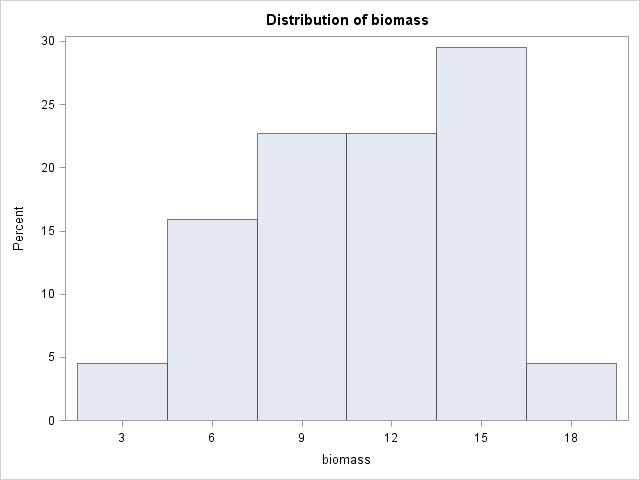
\includegraphics[scale=0.45]{biomasshist}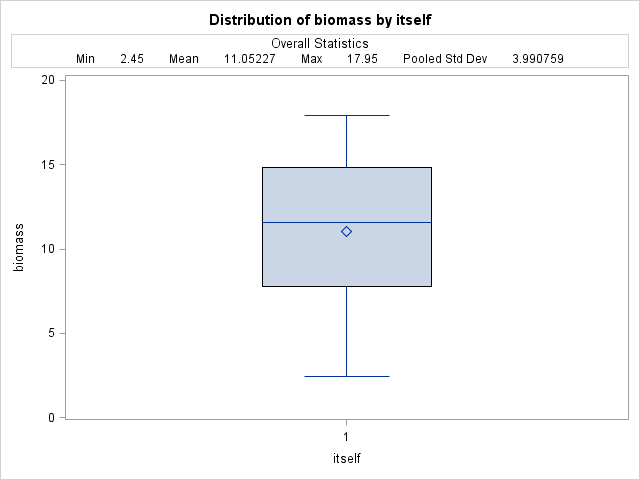
\includegraphics[scale=0.45]{biomassboxplot}\\
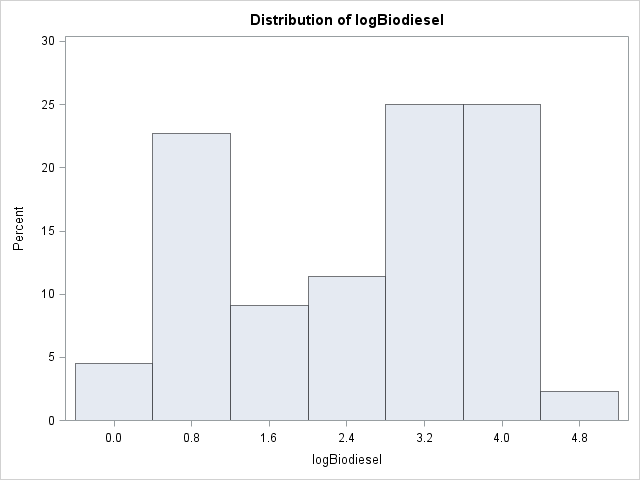
\includegraphics[scale=0.45]{logbiodieselhist}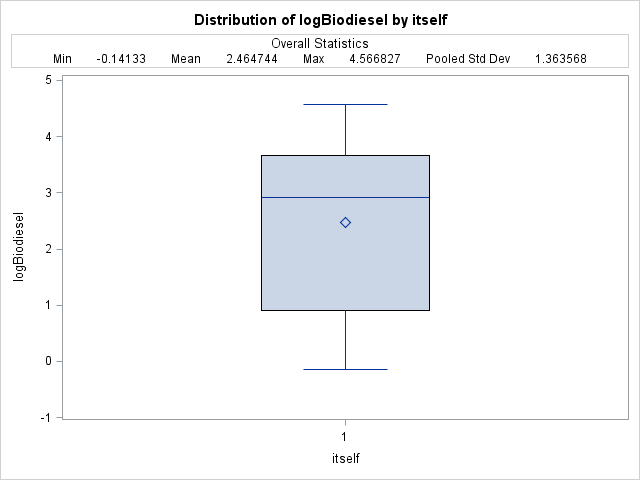
\includegraphics[scale=0.45]{logbiodieselboxplot}\\

How can we visually inspect the association between the two? A \textbf{Scatter plot} gives a visual approximation of the ``joint distribution'' between two variables.\\
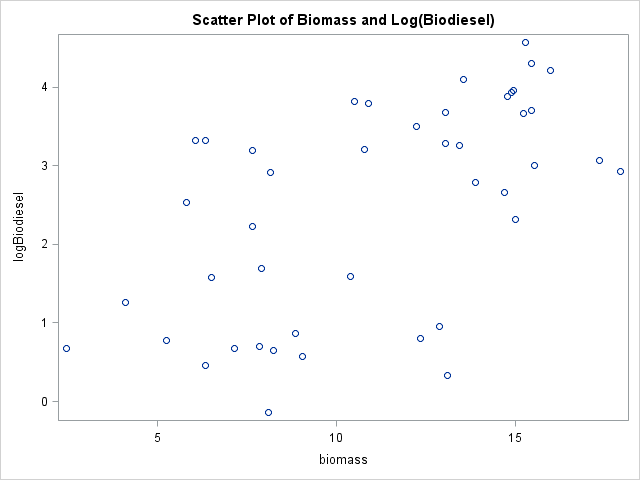
\includegraphics[scale=0.45]{scatterbiomasslogbiodiesel}\\~\\


\begin{flushright}
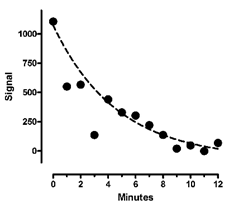
\includegraphics{scatternonlinear}
\end{flushright}

\newpage

\textbf{Properties of $r_{_{XY}}$}
\begin{itemize}
\item $r_{_{XY}}$ is an observed measure of the linear assn. between $X$ and $Y$ in a dataset.
\item correlation coefficient is unitless and always between -1 and 1:
$$ -1 \leq r_{_{XY}} \leq 1 $$
\item The closer $r_{_{XY}}$ is to 1, the stronger the positive linear association
\item The closer $r_{_{XY}}$ is to -1, the stronger the negative linear association
\item The bigger $|r_{_{XY}}|$, the stronger the linear association 
\item If $|r_{_{XY}}|=1$, then $X$ and $Y$ are said to be perfectly correlated (relationship is deterministic)
\end{itemize}
~\\
For the log(Biodiesel) (call this $Y$) and Biomass (call this $X$) example we can compute the sample correlation coefficient using summary statistics: \label{bio}
$$ \bar{x}=11.0523, ~~~~ s_X=3.9908, ~~~~\bar{y}=2.4647, ~~~~ s_Y = 1.3636$$ 
$$ s_{_{XY}}=\frac{\sum(x_i-\bar{x})(y_i-\bar{y})}{n-1} = 3.1485$$
Applying the formula for $r_{_{XY}}$, we get
$$ r_{_{XY}}=\frac{s_{_{XY}}}{s_X s_Y}=\frac{3.1485}{\sqrt{3.9908 \times 1.3636}} =0.5786$$

~\\~\\
Some example scatter plots\\
\begin{center}
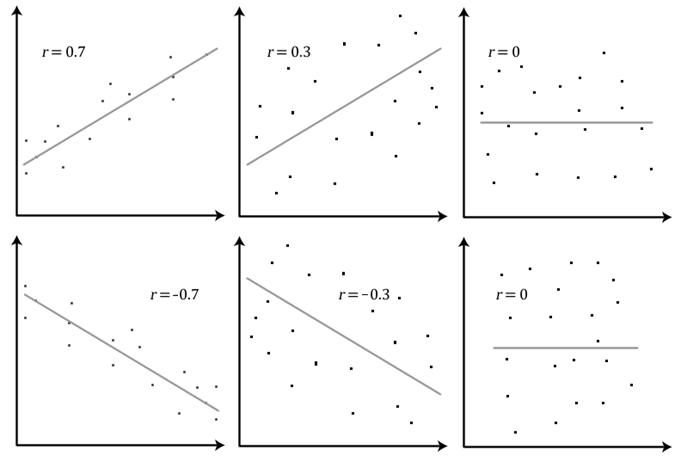
\includegraphics[scale=0.5]{scatterexamples}
\end{center}

\newpage
\cu{An exercise/activity:}
\noindent
Label the four plots below with the four sample correlation coefficients:
\begin{itemize}
\item $r=0.3$ ~~~~~~~~~~~~~~~~~~ $r=0.7$ 
\item $r=0.1$ ~~~~~~~~~~~~~~~~~~ $r=-0.6$ 
\end{itemize}
\begin{center}
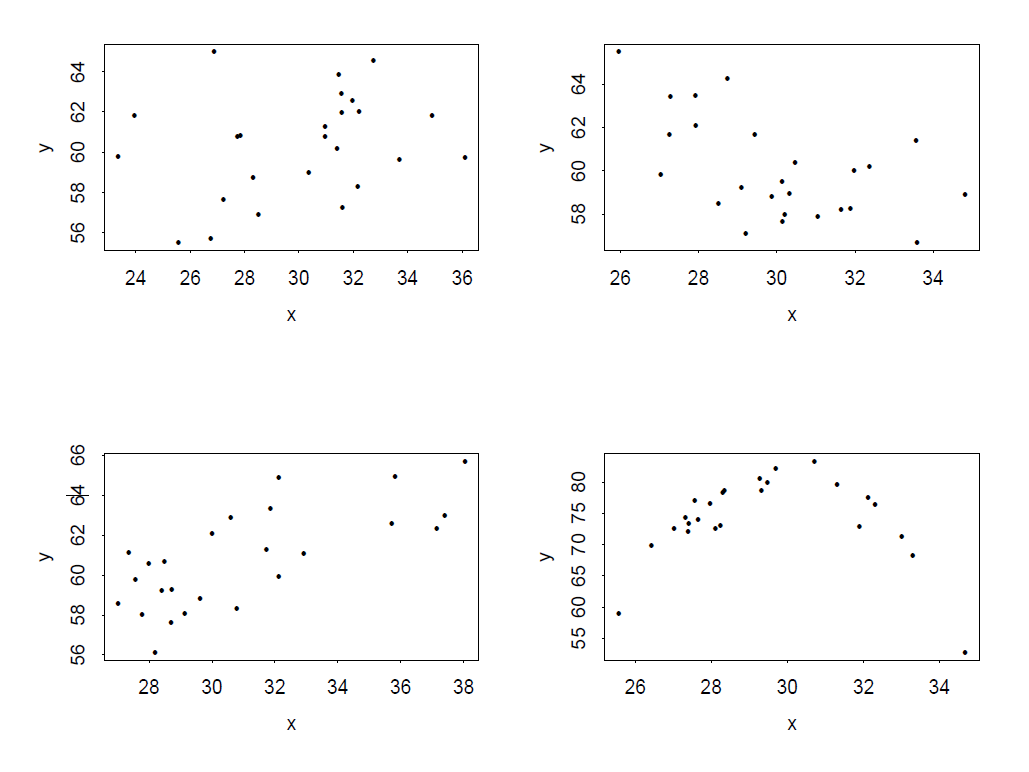
\includegraphics[height=3.5in,width=4.75in]{scattermatch}
\end{center}

Would it be appropriate to use correlation to summarize the relationship between age and pace in the following scatter plot?  Why or why not?
\begin{center}
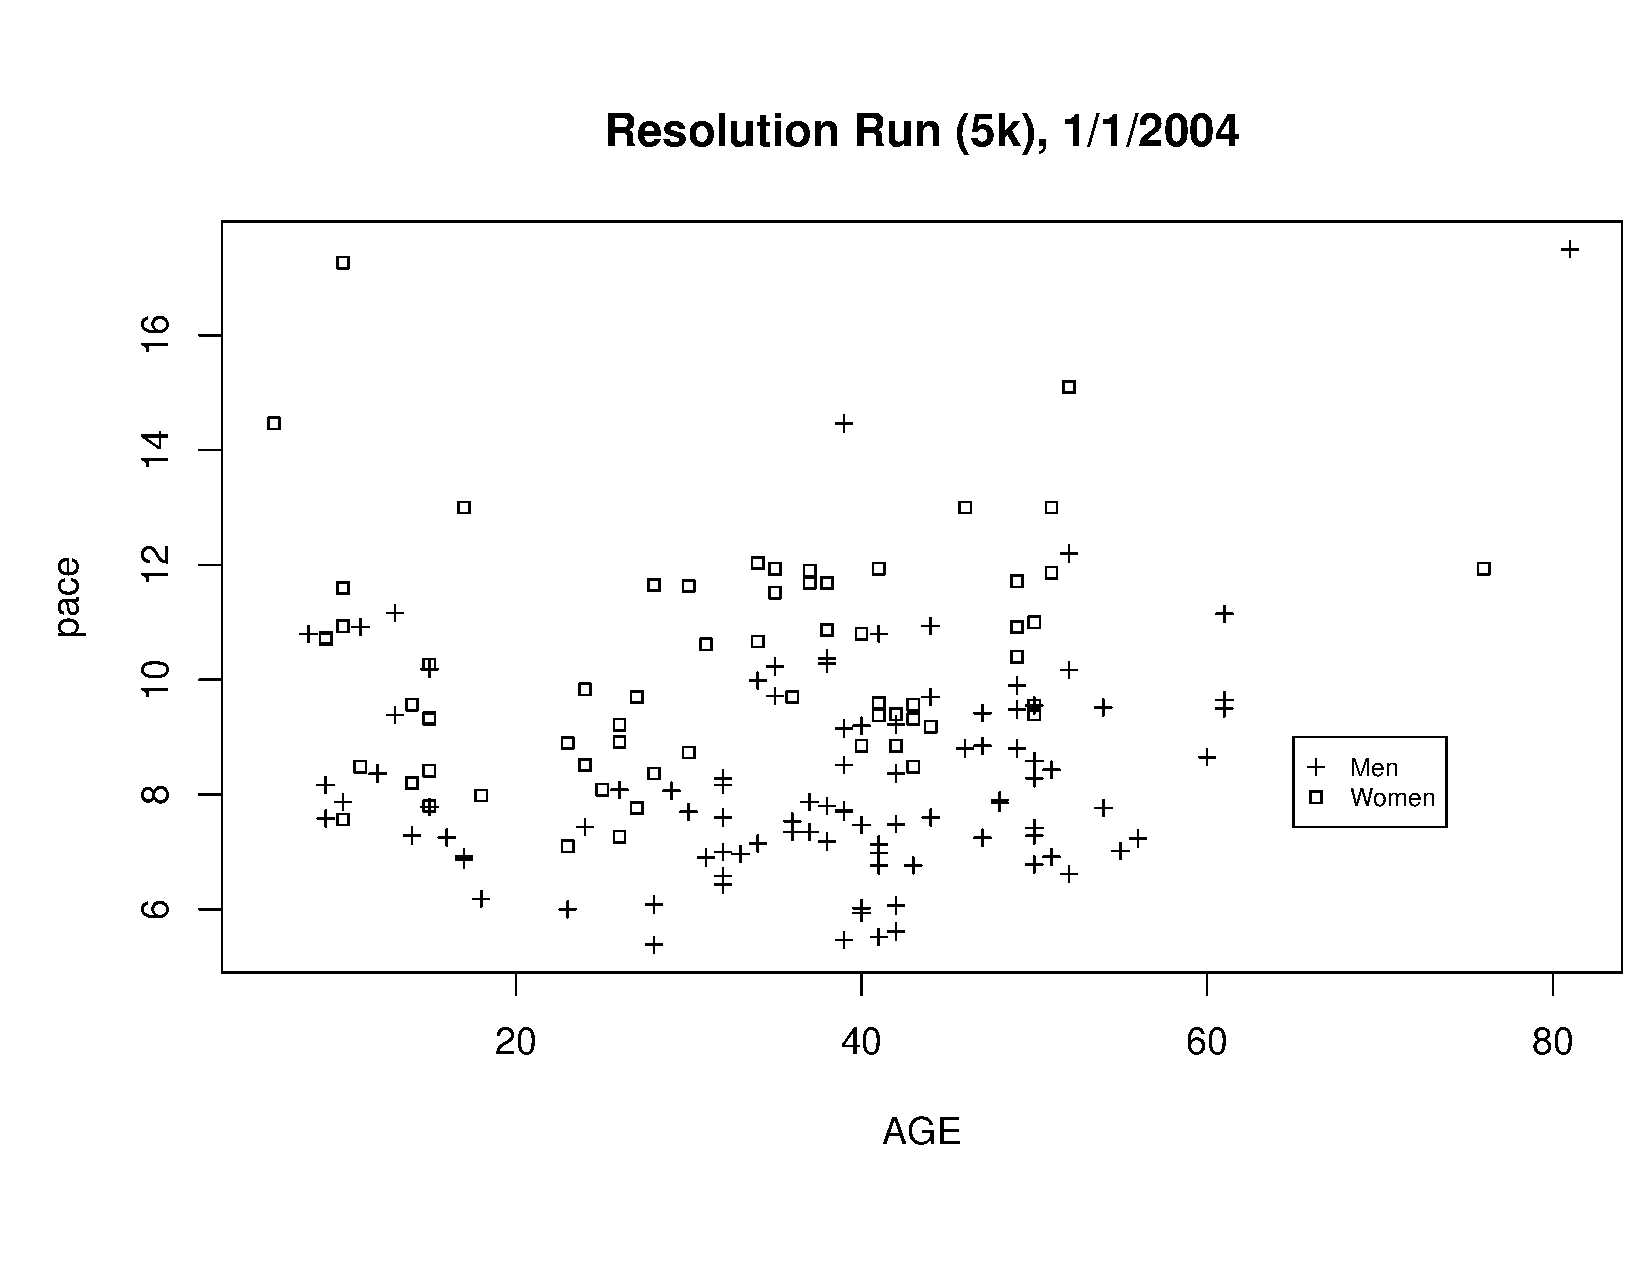
\includegraphics[height=3in,width=3.5in]{res5k_nomodel.pdf}
\end{center}

\textbf{To perform a Hypothesis Test about $\rho$:}\\
We often want to test the following hypotheses,
$$H_0:\rho=0 ~~~~~~~~H_A: \rho\neq 0$$
Assuming $H_0$ is true, the test statistic is 
$$z_{obs}=\left(\frac{1}{2}\sqrt{n-3}\right)\log \frac{1+r}{1-r}$$
and the reference distribution is the standard normal distribution, i.e. reject if $z_{obs}>z_{\alpha/2}$ or if $z_{obs}<z_{1-\alpha/2}$ where $z_{\alpha}$ satisfies $\alpha=\Pr(Z>z_{\alpha})$ with $Z\sim N(0,1)$.\\~\\
The p-value if found by finding $2P(Z>|z_{obs}|)$.  Why do we multiply by 2?\\~\\~\\

\textbf{To find a Confidence Interval for $\rho$:}\\
An approximate $100(1-\alpha)\%$ confidence interval for $\rho$ can be obtained by inverting the {\em Fisher transformation}:
$$ \left(\frac{\frac{1+r}{1-r}e^{-2z_{\alpha/2}/\sqrt{n-3}}-1}{\frac{1+r}{1-r}e^{-2z_{\alpha/2}/\sqrt{n-3}}+1}, \frac{\frac{1+r}{1-r}e^{2z_{\alpha/2}/\sqrt{n-3}}-1}{\frac{1+r}{1-r}e^{2z_{\alpha/2}/\sqrt{n-3}}+1}\right).$$

~\\~\\~\\
For the log(Biodiesel) and Biomass example our hypothesis test is:\\
$$H_0:\rho=0 ~~~~~~~~H_A: \rho\neq 0$$
$$\text{giving a test statistic of } z_{obs}=\frac{1}{2}\sqrt{44-3}~log\left(\frac{1+0.5786}{1-0.5786}\right)=4.228$$
Using an $\alpha=0.05$ our rejection region is any $z_{obs}$ outside of $\pm 1.96$.\\~\\
Our p-value $=2P(Z>4.228) = 2(0.00001) = 0.00002 < \alpha = 0.05$ so we reject our null hypothesis in favor of the alternative.\\~\\
What is the interpretation of the p-value=0.00002?\\
\indent The probability of getting a sample correlation (r) further (in magnitude) from 0 than 0.5786 assuming the true correlation ($\rho$) is 0 is 0.00002.\\~\\

\newpage

The corresponding 95\% confidence interval is 
$$\left(\frac{\frac{1+0.5786}{1-0.5786}e^{-2*1.96/\sqrt{44-3}}-1}{\frac{1+0.5786}{1-0.5786}e^{-2*1.96/\sqrt{44-3}}+1}, \frac{\frac{1+0.5786}{1-0.5786}e^{2*1.96/\sqrt{44-3}}-1}{\frac{1+0.5786}{1-0.5786}e^{2*1.96/\sqrt{44-3}}+1}\right) = (0.3401, 0.7471)$$
We can say that we are 95\% confident that the true correlation ($\rho$) is between 0.3401 and 0.7471.\\~\\
When we say confident, we mean that if we did this experiment repeatedly and made an interval for each experiment, the true correlation would fall in 95\% of the intervals created.\\~\\

\textbf{How can we get SAS to do this for us?}
\begin{small}
\begin{verbatim}
proc corr data=bioexp FISHER(biasadj=NO);
var butterfat temp;
run; 
\end{verbatim}
\end{small}

\begin{center}
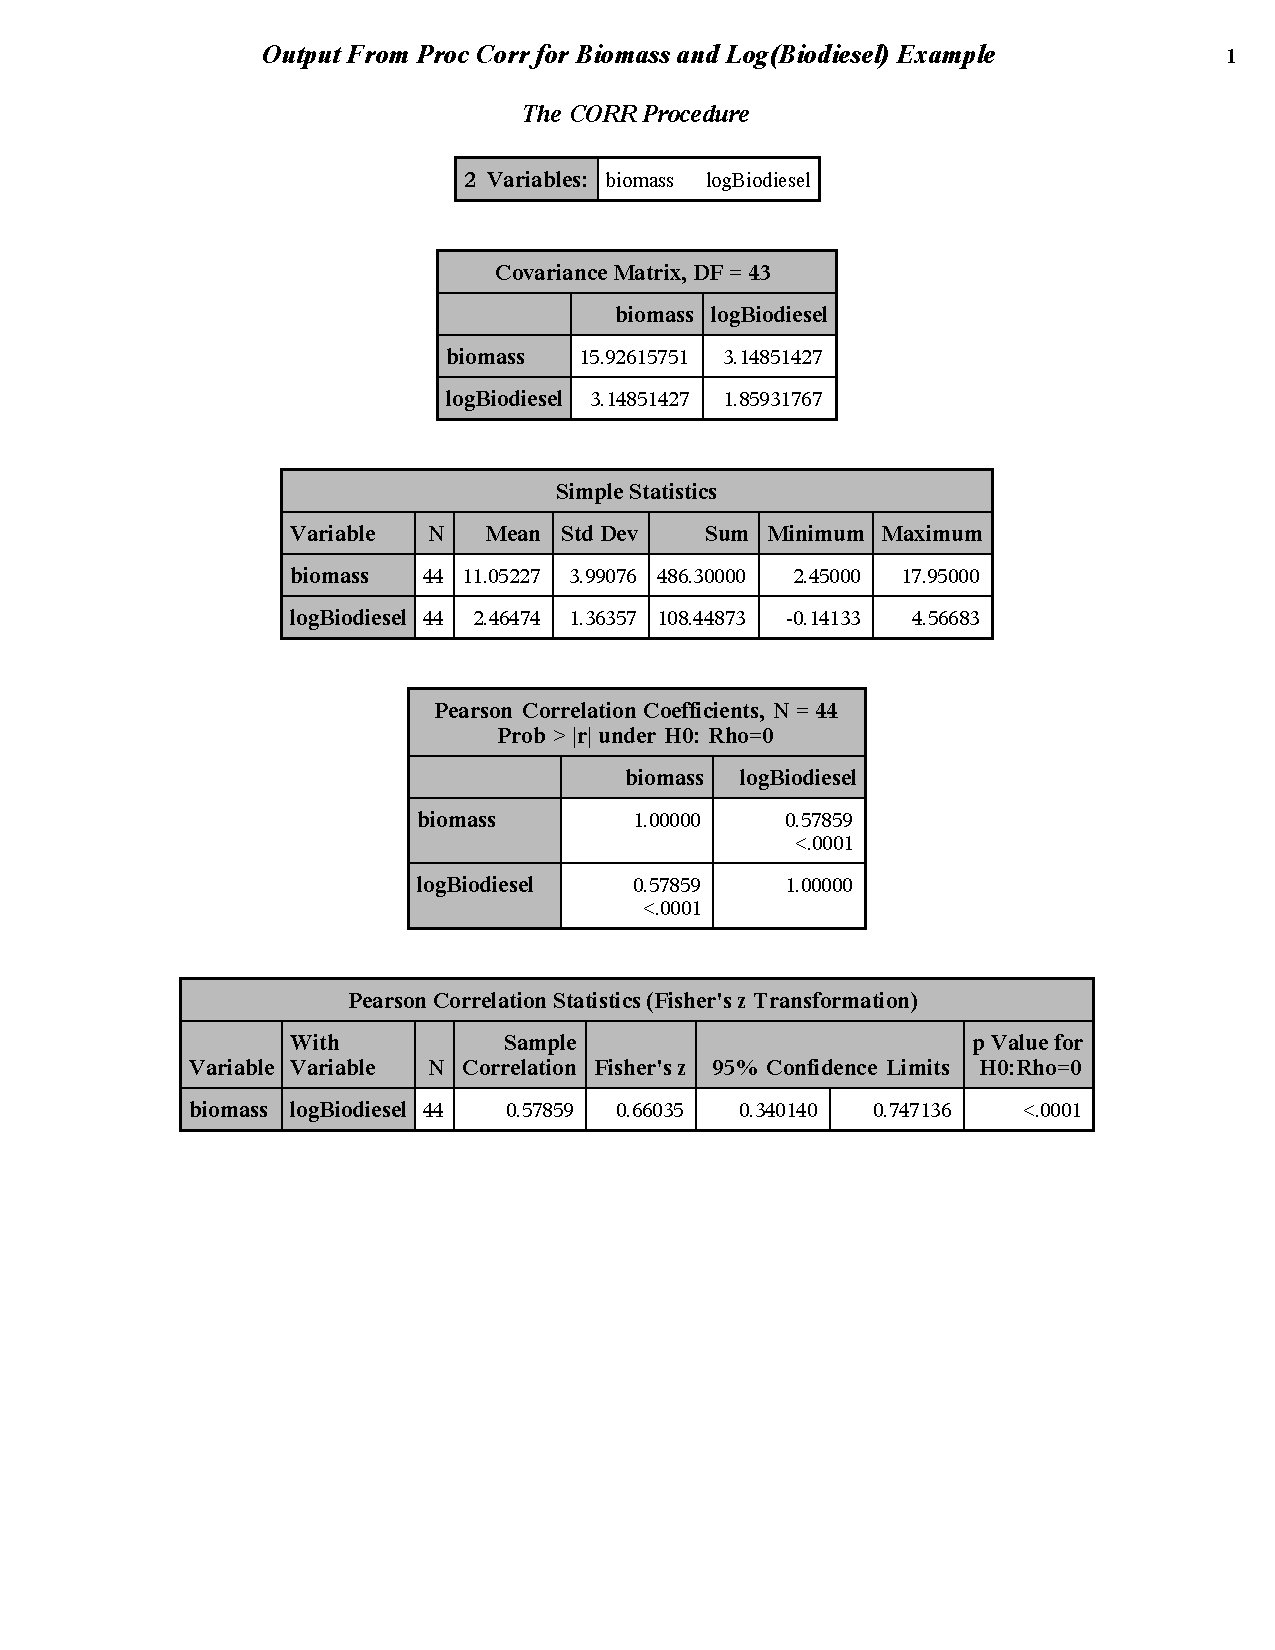
\includegraphics[scale=0.75,trim = 0mm 80mm 0mm 10mm]{corrbiodiesel.pdf}\label{corrbio}
\end{center}


\cu{Note:  Significant correlation does NOT imply causation}
Famous examples of {\em spurious correlations}:
\begin{itemize}
\item A study finds a high positive correlation between coffee drinking and coronary heart disease.  Newspaper reports say the fragrant essence of the roasted beans of {\em Coffea arabica} are a menace to public health.
\item In a city, if you were to observe the amount of damage and the number of fire engines for enough recent fires, you would likely see a positive and significant correlation among these variables.  Obviously, it would be erroneous to conclude that fire engines cause damage.
\item {\em Lurking variable} - a third variable that is responsible for a correlation between two others.  (A.k.a. confounding factor.)\\
An example would be to assess the association between say the reading skills of children and other measurements taken on them, such as shoesize.  There 
may be a statistically significant association between shoe size and reading skills, but that doesn't imply that one causes the other.  Rather, both are positively associated with a third variable, {\em age}.
\item Among 50 countries examined in a dietary study, high positive correlation among fat intake and cancer (see figure, next page).  This example is taken from from {\em Statistics} by Freedman, Pisani and Purves.\\~\\
\begin{quotation} 
In countries where people eat lots of fat like the United States rates of breast cancer and colon cancer are high. This correlation is often used to argue that fat in the diet causes cancer. How good is the evidence?

Discussion. If fat in the diet causes cancer, then the points in the diagram should slope up, other things being equal. So the diagram is some evidence for the theory. But the evidence is quite weak, because other things aren't equal. For example, the countries with lots of fat in the diet also have lots of sugar. A plot of colon cancer rates against sugar consumption would look just like figure 8, and nobody thinks that sugar causes colon cancer. As it turns out, fat and sugar are relatively expensive. In rich countries, people can afford to eat fat
and sugar rather than starchier grain products. Some aspects of the diet in these countries, or other factors in the life-style, probably do cause certain kinds of cancer and protect against other kinds. So far, epidemiologists can identify only a few of these factors with any real confidence. Fat is not among them. 
\end{quotation} 
(p. 152, {\em Statistics} by Friedman, Pisani, Purves and Adhikari)
\end{itemize}

\begin{center}
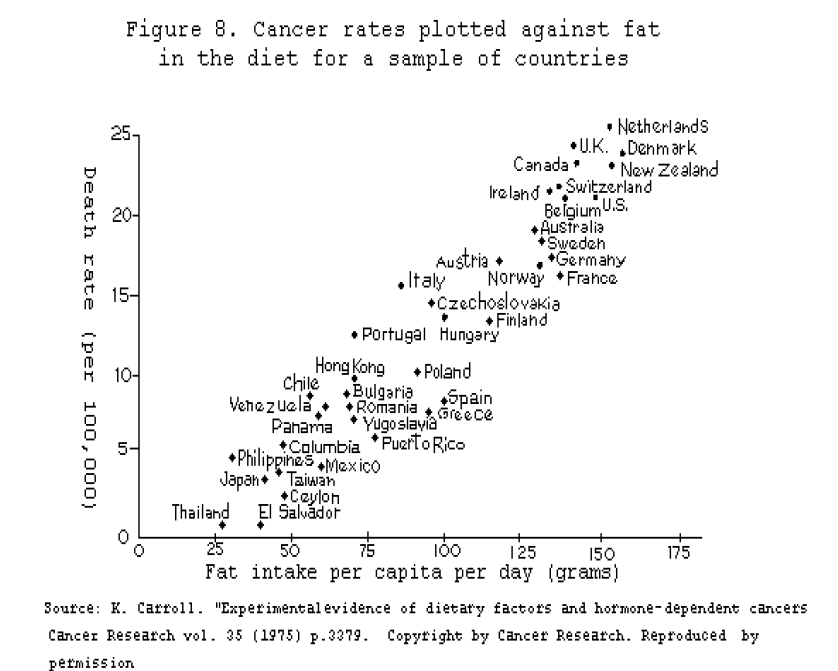
\includegraphics[scale=0.5]{scattercancer}
\end{center}








